\documentclass[12pt,a4paper]{article}
\usepackage{times}
\usepackage{durhampaper}
\usepackage{harvard}
\usepackage{graphicx}
\usepackage{tcolorbox}
\usepackage{wrapfig}
\usepackage{svg}
\usepackage{multirow}
\graphicspath{{images/}}

\citationmode{abbr}
\bibliographystyle{agsm}

\title{A Multiscale Data Storage Format and API}
\author{Dan Tuthill-Jones}
\student{D. Tuthill-Jones}
\supervisor{T. Weinzierl}
\degree{MEng Computer Science}

\date{}

\begin{document}

\maketitle

\begin{abstract}
\section*{Context/Background}
Much cutting-edge research such as the physics of earthquakes or modeling of astrophysical objects rely on the results of exceptionally large computational simulations. Those produced by the ExaHyPE project are 2D or 3D objects that can be too large for a standard computer to hold in memory or require an unreasonably long time to process for human consumption.

\section*{Aims}
A solution is required which allows for efficient rendering of low resolution samples of large datasets and interactive exploration of smaller areas of the dataset in higher resolutions.

\section*{Method}
This functionality is implemented as two pieces of software, the first of which is a standalone program that compresses the dataset and saves it to disk alongside the full resolution dataset. The second is a plugin for the visualisation software ParaView for compressing the dataset on the fly and exploring the dataset by selecting specific areas to load at higher resolution.

\section*{Results}
Small data files of around 400 MB in size can be sampled or rendered in aproximately 40 seconds. Larger data files that are around 6 GB in size cannot be rendered however they can be sampled to a low resolution in about 8 minutes and interactively exploring a selected area takes between 15 to 40 seconds.

\section*{Conclusion}
Through the combination of a multiscale data storage and an interactive visual exploration tool, it is possible to explore massive datasets in real time while maintaing the visual quality requirements.
\end{abstract}

\begin{keywords}
ParaView ExaHyPE Peano Multiscale File Format API Exascale Computing
\end{keywords}

\pagebreak
\section{Introduction}

The ExaHyPE (Exa-scale Hyperbolic PDE Engine) project \cite{exahype} seeks to address the software aspect of a supercomputer capable of performing a billion billion ($10^{18}$) operations per second or 1 exaflop/s. ExaHyPE focuses on the development of new mathematical and algorithmic approaches to exascale systems, initially applying the massive computational power to simulations in geophysics and astrophysics. The project integrates into Europe's strategy for developing an exascale supercomputer by 2020. The ExaHyPE project does not address the problem of visualizing the massive output datasets of exascale systems which can exceed the memory limitations of even specialized visualization workstations. This project aims to address this problem with post processing techniques to produce lower resolution versions of the dataset and allow interactive exploration of smaller areas in either higher or full resolution.

Under the hood of the ExaHyPE project is Peano \cite{Peano}. Peano is an open source C++ solver framework which embeds regular grids in a spacetree structure. Spacetrees are a generalisation of the 2D quadtree structure and the 3D octree structure. Quadtrees and octrees are used to partition space by recursively subdividing it into four and eight sections respectively. An example of octree partitioning is displayed in figure \ref{spacetree}.


\begin{figure}[h]
\centering
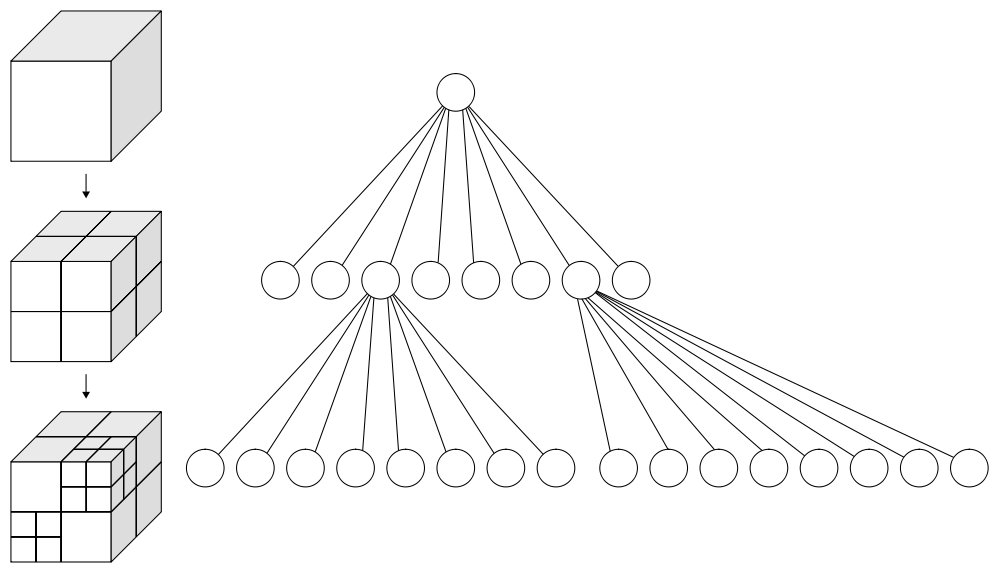
\includegraphics[scale=0.3]{1000px-Octree2}
\caption{The recursive partitioning of a cube by an octree}
\label{spacetree}
\end{figure}

Each leaf node in Peano's spacetree structure is a regular grid, also called a patch or Peano patch. Every regular grid has the same dimentionality and the size is dependant on its depth in the tree. The patches are used to further divide space in a memory-efficient way.
During a simulation, the spacetree structure allows for the computations on points in space to be performed at different resolutions i.e. levels of detail. In numerical analysis, this is called Adaptive Mesh Refinement \cite{DUBEY20143217}.
Peano realises a spacetree traversal and storage algorithm, and provides hook-in points for applications to perform per-element and per-vertex operations on the grid. It also provides interfaces for dynamic load balancing, sophisticated geometry representations, and other features. ExaHyPE is an implementation of a block-structured solver.


ParaView \cite{Paraview} is an open-source, multi-platform data analysis and visualization application. It was developed to analyze extremely large datasets using distributed memory computing resources. It can be run on supercomputers to analyze datasets of petascale size as well as on laptops for smaller data, has become an integral tool in many national laboratories, universities and industry, and has won several awards related to high performance computation.

The data files produced by Peano cannot be read by ParaView natively. Instead, Peano can write files to the native ParaView format, VTK. VTK does not support spacetree structure or other structrues with a lower memory footprint such as sets of regular grids. Therefore the dataset must be converted to an unstructured grid. Unstructured grids assume no underlying structure. The structure is explicitly defined within the file and therefore there is a larger memory footprint. This project aims to produce a plugin for ParaView which is capable of directly reading from the peano file format.

For many cutting edge simulation research projects, specifically the exa-scale problems tackled by ExaHyPE, the full resolution output data is so massive that it is not possible for even cutting edge visualisation hardware to process at a reasonable rate. Therefore traditional simulation visualisation methods follow a three step cycle. Step one is to run the simulation code. Step two is to visualize and step three is to adapt the plotting resolution of the output data. Then the cycle restarts and the simulation is run again. This project aims to modify the traditional cycle so that the simulation code only needs to be run once. This is achieved by adding a new step where lower resolution data is computed. A comparison of the two workflows is displayed in figure \ref{workflows}.

\begin{figure}[h]
\centering
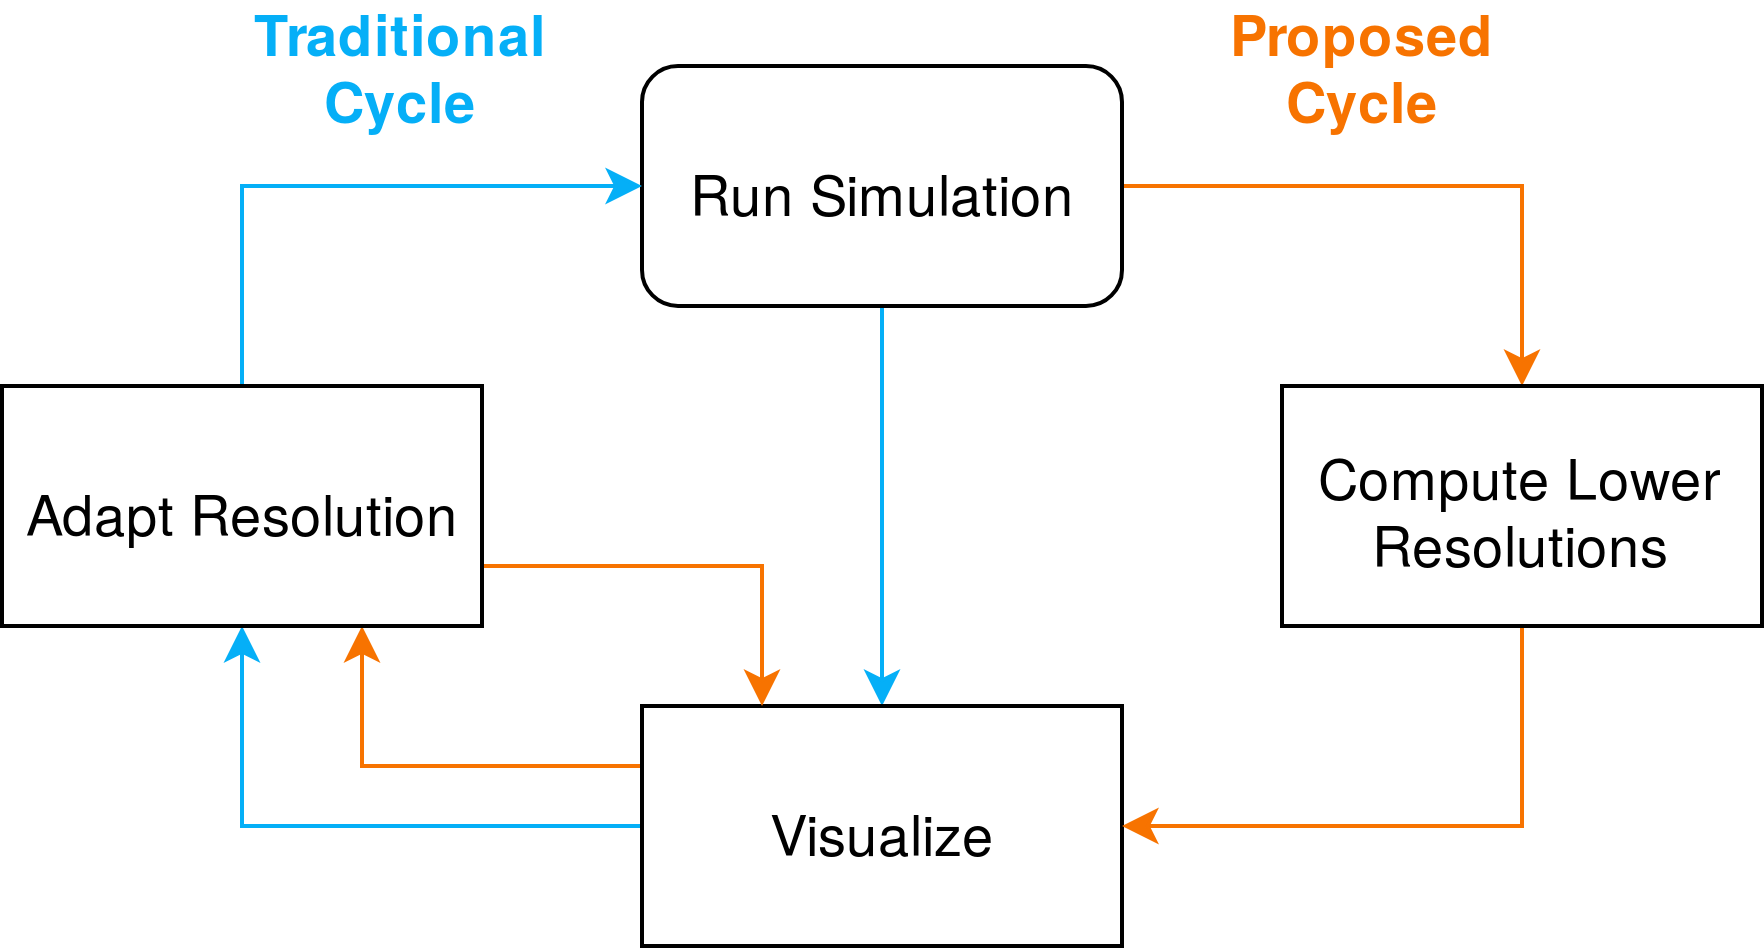
\includegraphics[scale=0.2]{vis-workflow}
\caption{A comparison of the traditional simulation workflow and our proposed workflow}
\label{workflows}
\end{figure}

The data produced by ExaHyPE is made up of many relatively small grids which we can sample on to a large, low resolution regular grid to produce a low resolution version of the dataset. This sampling technique will allow on the fly sampling via an interface of the paraview plugin and it will allow pre-computation of the lower resolution versions of the dataset via a standalone program. Finally, an interactive method of exploration shall be implemented so that the end user can select smaller specific areas to either apply the same sampling method or load full resolution data.

\section{Related Work}

\subsection{International Exascale Software Project Roadmap}
The International Exascale Software Project Roadmap \cite{Dongarra} was published in 2011. The purpose of the roadmap is to minimize the lost productivity due to lack of planning, coordination, and key integration of technologies necessary to make exascale computing technologies work together smoothly and efficiently. Millions of dollars and years of work have already been invested into exascale computing technologies and there is only going to be more investment in the future. A roadmap is needed because a completely uncoordinated development model will not provide the required software for the massive parallelism for exascale computation by 2020. Additionally it is important that the developers of new exascale technology are aware of the benefits of new hardware models and features such as transactional memory \cite{TransMemory} and speculative execution \cite{ValuePredictionTechniques}.

The IESP splits the goal of Exascale computing in to the following sequence of five objectives and tackles the first two.

\begin{enumerate}
\item Make a thorough assessment of needs, issues and strategies
\item Develop a coordinated software roadmap
\item Provide a framework for organizing the software research community
\item Engage and coordinate with the vendor community in cross-cutting efforts
\item Encourage and facilitate collaboration in education and training
\end{enumerate}

The International Exascale Software Project Roadmap provides separate timeframes for the completion of individual targets in many software areas. Each software area belongs to one of four groups; System Software, Development Environments, Applications and Cross-cutting Dimensions. System Software contains operating systems, runtime systems, I/O systems, systems management and external environments. Development Environmnts contains programming models, frameworks, compilers, numerical libraries and debugging. Applications contains algorithms, data analysis, visualisation and data management. Cross-cutting Dimensions contains resilience, power management, performance optimisation and programmability. 

%\subsection{Block-Strcuted solvers}
%A survey of high level frameworks in block-structured adaptive mesh refinement packages


\subsection{SCI Run}
SCIRun \cite{SCI:SCIRun} which is produced by the Scientific Computing and Imaging Institute at the University of Utah and was first released in 1999. Researchers use SCIRun to create a high level workflow through its visual programming environment for visualization, modeling and simulation. SCIRun does have some multiresolution functionality. It is capable of computing lower resolution models on the fly and exploring specific areas in higher resolution however it does not support precomputation of the lower resolutions \cite{SCIRun2}.

\subsection{VisIt}
After the release of a proptype in 2000, in 2002 The Department of Energy (DOE) Advanced Simulation and Computing Initiative (ASCI) released VisIt \cite{VisIt}. VisIt is an open source interactive parallel visualization and graphical analysis tool for viewing scientific data. It can be used to visualize scalar and vector fields defined on 2D and 3D structured and unstructured meshes. VisIt was originally developed to visualize and analyze the results of terascale ($10^{12}$) simulations. It was designed with a high degree of modularity to support rapid deployment of new visualization technology. Like ParaView, VisIt includes a plugin architecture for custom readers, data operators and plots as well as the ability to support multiple different user interfaces.

\subsection{ExaHyPE directly writing to VTK}
ExaHyPE is capable of directly writing its output data to the VTK format however this has some issues. VTK does not natively support a format i.e. spacetrees or sets of patches. This means the memory footprint is increased because the position of every data point has to be stored instead of being calculated using the index. The VTK reader does not support metadata files, therefore if MPI \cite{MPI} is used and the data for a single dataset is spread accross multiple files, the data will need to be combined into a single file at a later date. Additionally, the lack of metadata files means that the loading of pre-computed lower resolution data cannot be integrated into a ParaView interface. The sampling techniques that are implemented in the project rely on the Peano Patch structure and so to apply them onto a VTK dataset would require additional computation to convert the files to Peano Patches.

\subsection{Peano File Format}
The output of the Peano Solver Framework is split into Peano Metadata files and Peano Patch files. The Metadata files define the datasets in a time series and the Peano Patch files contain the actual data.

\subsubsection{Peano Metadata Files}
Metadata files link 1 or more patch files into a single dataset and combine multiple datasets into a time series. There may be multiple patch files per dataset. This is because MPI \cite{MPI} can be used by Peano to distribute the workload over multiple computational nodes. In this case, each MPI rank writes to its own file and the resulting dataset is the union of all data contained in that dataset's files. See figure \ref{metadata-original} for an example Peano Metadata file.

\begin{figure}[h]
\begin{tcolorbox}
\# \\
\# Peano metadata output file \\
\# Version 0.2 \\
\# \\
format ASCII \\
\\
begin dataset \textbf{\textit{\# Element 0 in the time series}} \\
\null\quad include Simulation-0-rank-0.peano-patch-file \textbf{\textit{\# 0th Patch file for this dataset}} \\
\null\quad include Simulation-0-rank-1.peano-patch-file \textbf{\textit{\# 1st Patch file for this dataset}} \\
end dataset \\
 \\
begin dataset \textbf{\textit{\#Element 1 in the time series}} \\
\null\quad include Simulation-1-rank-0.peano-patch-file \textbf{\textit{\# 0th Patch file for this dataset}} \\
\null\quad include Simulation-1-rank-1.peano-patch-file \textbf{\textit{\# 1st Patch file for this dataset}} \\
end dataset
\end{tcolorbox}
\caption{A Peano Metadata file with two datasets and four patch files}
\label{metadata-original}
\end{figure}

\subsubsection{Peano Patch Files}
Although the internal format used by Peano is that of a spacetree, Peano patch files define a set of cartesian grids. Each grid is called a patch. The reason a spacetree is not used is that when ExaHyPE is ran on a HPC using MPI, each MPI rank writes to its own file and it is difficult to maintain a spacetree structure accross multiple files. At the start of the file, the number of dimensions and size in each dimension is defined. All patches in the file have these properties. Next, the variables are defined by name. Each variable can either be defined on the vertices or the cells of the patch. Each variable also defines the number of unknowns which is the number of values stored per element. Optionally, a variable will define mapping values. The mapping values define the positions of each vertex inside the patch by relative values between 0 and 1. Finally the patches themselves are defined. Each patch defines its size and offset from the origin and the actual values for each variable are defined by double precision floating point numbers. An example Peano Patch file with a single patch and two variables can be found in figure \ref{patch-file}

\begin{figure}[h!]
\begin{tcolorbox}
\# \\
\# Peano patch file \\
\# Version 0.2 \\
\# \\
format ASCII \\
dimensions 3 \\
patch-size 3 3 3 \\
 \\
begin cell-values "Magnitude" \\
\null\quad number-of-unknowns 1 \\
end cell-values \\

begin cell-values "Directon" \\
\null\quad number-of-unknowns 3 \\
end cell-values \\
 \\
begin patch \\
\null\quad offset 0 0 0 \\
\null\quad size 1 1 1 \\
\null\quad begin cell-values "Magnitude" \\
\null\quad\quad 1 1 1 1 1 1 1 1 1 1 1 1 1 1 1 1 1 1 1 1 1 1 1 1 1 1 1 \\
\null\quad end cell-values \\
\null\quad begin cell-values "Direction" \\
\null\quad\quad 1 0 0 1 0 0 1 0 0 1 0 0 1 0 0 1 0 0 1 0 0 1 0 0 1 0 0 1 0 0 1 0 0 1 0 0 1 0 0 1 0 0 1 0 0 1 0 0 1 0 0 1 0 0 1 0 0 1 0 0 1 0 0 1 0 0 1 0 0 1 0 0 1 0 0 1 0 0 1 0 0 \\
\null\quad end cell-values \\
end patch
\end{tcolorbox}
\caption{A Peano Patch file with two three-dimensional patches}
\label{patch-file}
\end{figure}

\section{Solution}
\subsection{Overview}
Our solution is implemented as two pieces of software. The first is a standalone program. This software can convert the output files of Peano/ExaHyPE to vtk, the native file format for ParaView. Alternatively, it can sample the datasets onto regular grids so that lower resoltion data can be loaded from the disk instead of computed on the fly.

The second piece of software is a plugin for the visualisation software ParaView. This plugin allows ParaView to directly read Peano/ExaHyPE's output files, perform sampling on the fly, load precomputed datasets and explore the dataset by selecting specific areas to load at higher resolution. The intended use of this software is as follows:

\begin{itemize}
\item An ExaHyPE simulation is run producing some full resolution output data
\item The standalone program is run on the dataset, producing some low resolution versions of the dataset
\item The metadata file is opened in ParaView with the plugin installed
\item The user opens the low resolution data which was precomputed earlier
\item The user uses the interactive box to select an  area of intrest to load in higher resolution
\item The user uses the interactive box to further load areas of intrest in high resolution.
\end{itemize}

\subsection{Data Representation Layer}

%\begin{wrapfigure}{r}{0.25\textwidth}
%    \centering
%	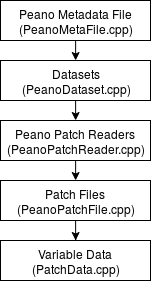
\includegraphics[scale=0.8]{data-representation-small}
%	\caption{The software structure of the data representation layer}
%\end{wrapfigure}

The data representation layer concerns the conversion of Patch files to C++ objects containing the same data. The C++ objects that form this layer maintain the same hierarchical structure as the data files. The layers of this structure are as follows:

\begin{enumerate}
\item The top layer is the $PeanoMetaFile$ object. This reads and parses the data of the Peano Metadata file.

\item The $PeanoMetaFile$ object generates the second layer by creating a $PeanoDataset$ object for each element in the time series. Each $PeanoDataset$ object is instantiated with the list of Peano Data files that contain its data.

\item When a program requests a dataset, it also requests which of the available resolutions to load. The $PeanoDataset$ object then creates a $PeanoReader$ for every file in the dataset at that resolution. The $PeanoDataset$ objects read the Peano Patch data into a set of $PeanoPatch$ objects.

\item The actual vertex and cell data is held in $PatchData$ objects. One instance per $PeanoPatch$.
\end{enumerate}

\subsection{Conversion of Patch objects to VTK Objects}
The conversion of a single Peano Patch to a VTK object is straightforward. A regular Peano patch is equivalent to VTK's $vtkImageData$ object. The position, size and dimention information which is held in the $PeanoPatch$ object can be passed directly to a vtkImageData instance. The cell and vertex data held in the $PeanoData$ objects can then be used to create a $vtkDoubleArray$ which is then passed to the $vtkImageData$ object.

Conversion of a Peano Patch with mapping data is a little more complicated. Because no positional structure is guarenteed the object must be converted to a $vtkUnstructuredGrid$. The same process for the regular grid is performed except the $vtkUnstructuredGrid$ is passed a $vtkPointArray$ initialized with the positional data.

The previosuly outlined processes converts a single $PeanoPatch$ object to a VTK oject however the full resolution dataset is a set of these objects. Conveniantly, VTK provides us with the $vtkAppendFilter$ object. We use this object to combine the individual VTK objects to produce a $vtkUnstructuredGrid$ containing all the input datasets.

\subsection{Sampling}

\subsubsection{Mapping}
To reduce the resolution of the output data, a sampling method is used to map values from the original full resolution output data on to a lower resolution regular grid. We can either sample onto a grid which covers the entire dataset or we can use a ParaView 3D widget to select a specific region of the dataset to sample onto.
Internally, the regular grid is a single Peano Patch object. This allows any Peano patch operations to be performed on it.

The single dimentional mapping of a point in the input dataset to the index of a point of the regular grid is
\[
	index = \frac{resolution\times(position - offset)}{size}
\]

Where $resolution$ is the number of points in the grid, $offset$ is the offset of the regular grid, $position$ is the position of the data point and $size$ is the size of the regular grid.

\subsubsection{Sampling Methods}
The three sampling methods available to us are

\begin{itemize}
\item Mapping each point onto the regular grid and taking the last values at each point
\item Mapping each point onto the regular grid and taking the average of the values at each point
\item Mapping each point onto the regular grid and taking the weighted average at each point depending on the certesian distance from the landing point
\end{itemize}

All three methods use the same time complexity of $O(n)$ where $n$ is the size of the input, however the first is the most performant because there is no calculation of averaging or weighting and no additional memory is required. The second two methods both require $O(n)$ space complexity. Because of the performance benefit, we decided to implement the first method.

\begin{figure}[h]
\centering
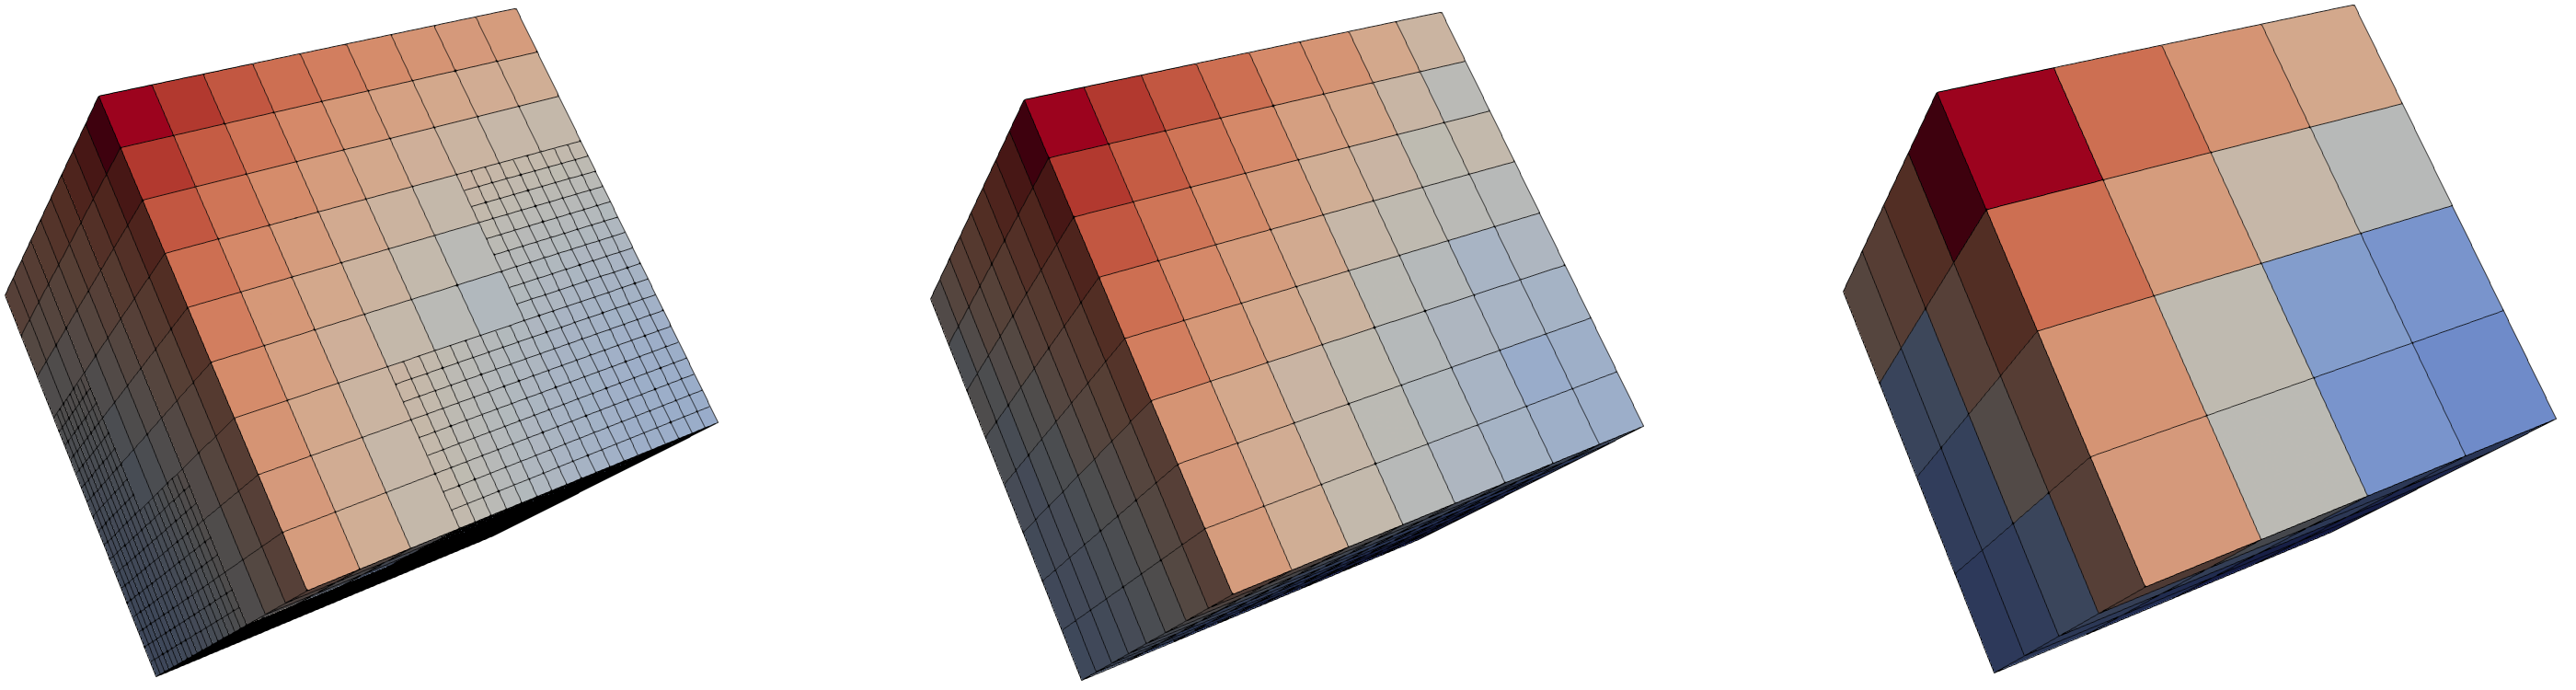
\includegraphics[scale=0.15]{three-cubes}
\caption{A full resolution dataset, an 8x8x8 dataset and a 4x4x4 dataset.}
\label{three-cubes}
\end{figure}

\subsubsection{Spacetree based sampling}

If the spacestree structure was maintained within the Peano Patch file format, then we could reduce the resolution through tree operations. Sets of leaf siblings can be removed by sampling their values onto their parent node. In figure \ref{spacetree-decimation} the decimation process is displayed. For this method, the lowest leaf nodes are removed and sampled onto the parent by taking the average values of the children nodes. The advantage of tree operations is that the tree structure is maintened so you efficiently reduce the resolution of the data while maintaining the high and low detail areas already present. This could not be implemented because the spacetree structure is lost when saving to Peano Patch files.

\begin{figure}[h]
\centering
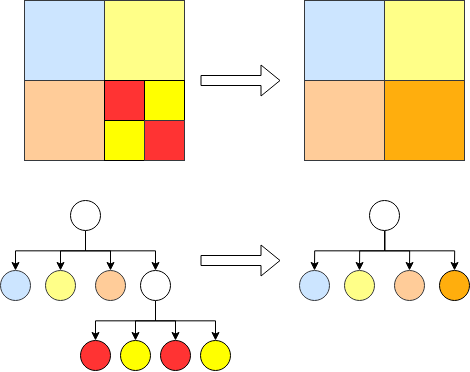
\includegraphics[scale=0.5]{spacetree-collapse}
\caption{The spacetree decimation process}
\label{spacetree-decimation}
\end{figure}

\subsection{Integration of Multiscale Datasets}
The lower resolution datasets are integrated into the Peano File format by referencing them in the Metadata File. In the metadata file, a dataset starts with the line $begin dataset$ and ends with the line $end dataset$. Peano Data files are included in the dataset by the $include$ statement, followed by the name of the file. Lower resolution variants of the data are included by adding the resolution, seprated by spaces after the include statement. When the $DataSet$ object is saved, it appends the resolution in brackets to the file name of the first full resolution file. See figure \ref{metadata-new} for an example.

\begin{figure}[h]
\begin{tcolorbox}
\# \\
\# Peano metadata output file \\
\# Version 0.2 \\
\# \\
format ASCII \\
\\
begin dataset \textbf{\textit{\# Element 0 in the time series}} \\
\null\quad include out-0.peano-patch-file \textbf{\textit{\# Full resolution data}} \\
\null\quad include 10 10 10 out-0-(10-10-10).peano-patch-file \textbf{\textit{\# 10x10x10 resolution data}} \\
end dataset \\
 \\
begin dataset \textbf{\textit{\# Element 1 in the time series}} \\
\null\quad include out-1.peano-patch-file \textbf{\textit{\# Full resolution data}} \\
\null\quad include 10 10 10 out-1-(10-10-10).peano-patch-file \textbf{\textit{\# 10x10x10 resolution data}} \\
end dataset
\end{tcolorbox}
\caption{A Peano Metadata file with two datasets and two resolutions per dataset}
\label{metadata-new}
\end{figure}

\subsection{ParaView Plugin}
It is possible to extend the function of ParaView through the use of plugins. There are different types of plugins such as sources and filters however we require a file reader. A ParaView Reader is a C++ object which ParaView interacts with. When a file is first loaded, ParaView performs an intial information request function call on the reader. Here information such as the number of datasets in the timeseries is passed to ParaView. After the information request, ParaView will request VTK data objects at specific times and load them in to its visualizer.

\subsubsection{Workflow}

\begin{figure}[h]
\centering
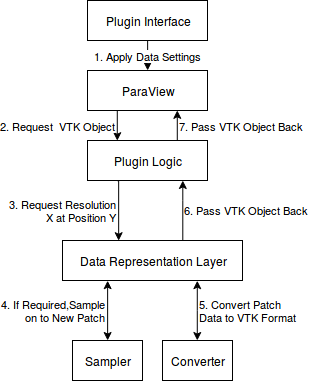
\includegraphics[scale=0.7]{solution-workflow}
\caption{The workflow of the ParaView plugin}
\end{figure}

\subsubsection{User Interface}

The user interfaces for ParaView Plugins are implemented through a combination of XML and C++ code. The XML is used to define the user interface elements and the C++ code handles the logic behind them. A checkbox is used to switch between sampling on the fly and loading directly from the disk. When the user is sampling, they can select the new resolution using the "Sample resolution" value boxes. The resolution to load box selects the precomputed resolution to sample from. This allows the user to prioritize the speed of the sampling by selecting a lower resolution or prioritize the accuracy by selecting a higher resolution.

If the "Explore Area" is set to none, then the sampling takes place over a new patch which minimally covers the entire dataset. The other option for the explore area presents the user with an interactive selection box. If on the fly sampling is enabled, then the data is sampled onto a patch covering this exact area. If on-the-fly samling is unselected, then all patches that are inside or overlap with the box are included. Any resolution selection is ignored because the precomputed resolutions are stored as a single patch and therefore with this method only all or nothing can be included. The advantage of this, is that the output 3D object is smaller and also the Patch reader will skip reading a patch if it is found to not lie within the selected range. This significantly increases the read performance.

\begin{figure}[h]
\centering
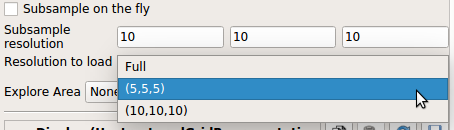
\includegraphics[scale=0.6]{paraview-interface-small}
\caption{The Plugin's ParaView Interface}
\label{ParaView-interface}
\end{figure}

The dataset can be explored by selecting an area with the interactive selection box shown in figure \ref{interactive-box}. This box has 6 grabbable nodes, one in the centre of each face. Dragging on these nodes will extend or retract the box in that direction. Another node is found at the centre of the box and dragging this allows the user to move the box around the dataset. Additionally, the box parameters can be entered manually in the box interface shown in figure \ref{box-manual}.

\begin{figure}[h]
\centering
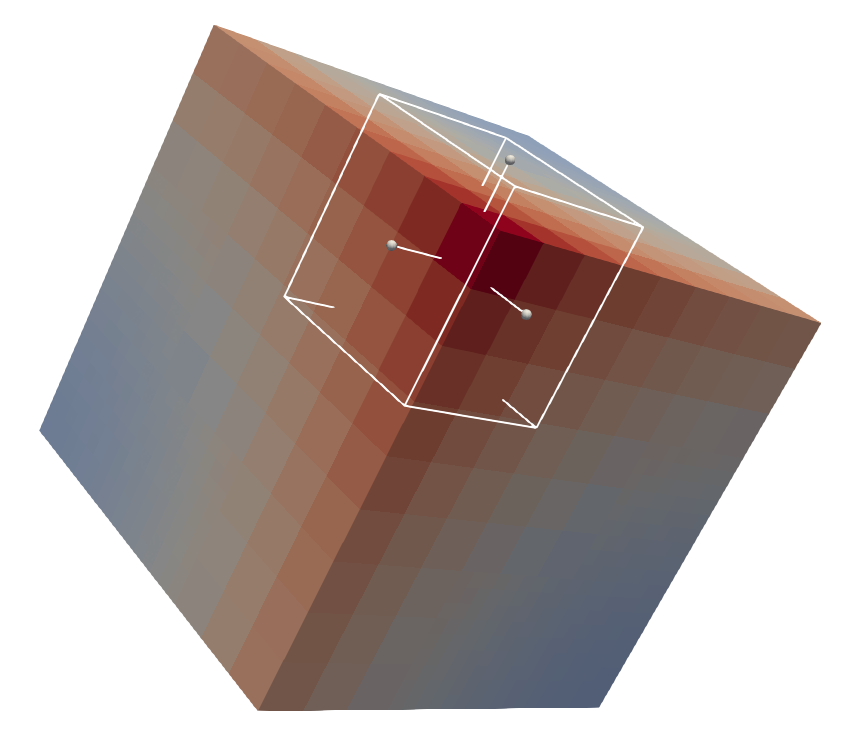
\includegraphics[scale=0.3]{area-select-2}
\caption{The interative explore box used to select areas of the dataset in ParaView}
\label{interactive-box}
\end{figure}

\begin{figure}[h]
\centering
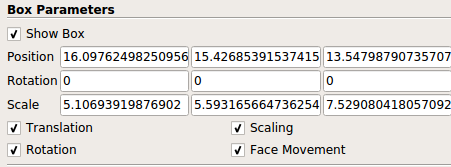
\includegraphics[scale=0.6]{box-params}
\caption{The parameter interface of the exploration box}
\label{box-manual}
\end{figure}

\section{Results}
\subsection{Generating Test Data}
To generate some test data, a tool was created which generates Peano Patch files. This tool creates patches in the shape of a regular grid where every cell is a 3 dimentional patch of size 3x3x3. There is also a single variable and every value is set to a random double value. The number of patches in each direction and the number of unknowns of the variable can be changed to increase or decrease the file size. The tool can generate patch files of any size by changing the number of patches and the number of unknowns.

All tests were run on a laptop with the following main components. CPU: Intel i5-2520M (2 cores, 4 threads, 2.5GHz with TurboBoost to 3.2GHz, 3MB cache). RAM: 8GB 1333MHz CL9. Storage: Samsung Evo 850 250GB SSD. This is a relatively old system that was released in 2011 and only the SSD has been replaced. There is no dedicated graphics card.

\subsection{Performance of Standalone}
For the first tests, the number of unknowns was set to 20 and the number of patches was varied in order to change the size of the input dataset. It is important to note that this test was performed on a single patch and so the standalone's parallelism is not used. Additionally, the size of the output patch was maintained at 20x20x20 because its size does not have a significant impact on the computation time. The size of the output patches were all approximately 1.7MB. The results are shown in table \ref{standalone-table}

\begin{table}[h]
\centering
\begin{tabular}{rrr}
\hline
\multicolumn{1}{l}{Total Patches} & \multicolumn{1}{l}{File Size} & \multicolumn{1}{l}{Time (Seconds)} \\ \hline
15 625                            & 390 MB                         & 39.323                             \\
27 000                            & 670 MB                        & 64.837                             \\
64 000                            & 1.6 GB                        & 142.783                            \\
125 000                           & 3.1 GB                        & 300.724                            \\
216 000                           & 5.4 GB                        & 478.439                            \\ \hline
\end{tabular}
\caption{The time taken to sample various datasets on to a 20x20x20 grid}
\label{standalone-table}
\end{table}

Plotting these test results on a graph (Figure \ref{standalone-time-graph}) shows that the time taken to sample the dataset onto a smaller patch is roughly linearly proportional to the size of the patch file (both in terms of file size and number of patches since they are linearly proportional).

\begin{figure}[h]
\centering
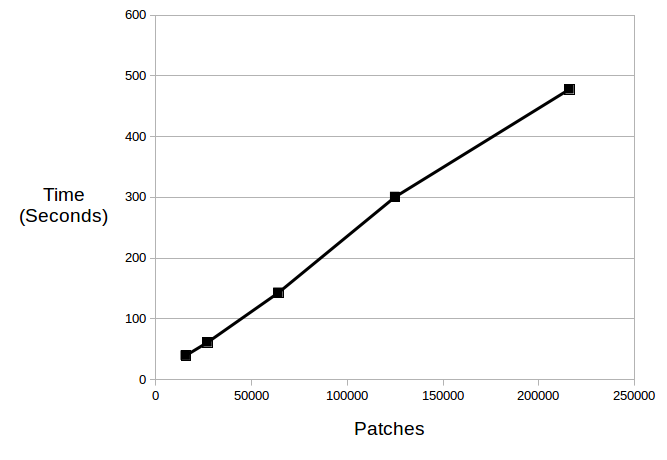
\includegraphics[scale=0.8]{standalone-time-graph2}
\caption{A graph of the time taken to sample various datasets on to a 20x20x20 grid}
\label{standalone-time-graph}
\end{figure}

\subsection{Performance of Reading Patch Files}
This test used the same data files as used for the standalone performance test. The 15 625 patch file (390 MB) loaded in to ParaView in 60.9 seconds and the 27 000 patch file (670MB) loads in 103.5 seconds however the 64 000 patch file (1.6 GB) could not be loaded because of an out of memory exception.

\subsection{Exploration Time}
This test used the same data files as used previously. The area of the selection box was changed to select different number of patches. The data collected can be found in table \ref{explore-graph}.

\begin{table}[h]
\centering
\begin{tabular}{rrrr}
\hline
\multicolumn{1}{l}{\multirow{2}{*}{Patches in File}} & \multicolumn{3}{c}{Time to Load (Seconds)}                                                              \\
\multicolumn{1}{l}{}                                 & \multicolumn{1}{l}{15625 Patches} & \multicolumn{1}{l}{8000 Patches} & \multicolumn{1}{l}{3375 Patches} \\ \hline
15625                                                & 65.0                              & 33.7                             & 16.4                             \\
27000                                                & 67.3                              & 34.3                             & 17.0                             \\
64000                                                & 71.5                              & 35.6                             & 21.5                             \\
125000                                               & 88.1                              & 37.5                             & 28.6                             \\
216000                                               & 112.0                             & 46.2                             & 40.3                            
\end{tabular}
\caption{The time taken to load a varying number of patches from different size files}
\label{explore-graph}
\end{table}

Plotting the results on a graph (figure \ref{explore-graph}). Shows that the time taken to load a selection of patches is linearly proportional to the number of patches selected and also that there is a significant overhead which is roughly proportional to the size of the patch file.

\begin{figure}[h]
\centering
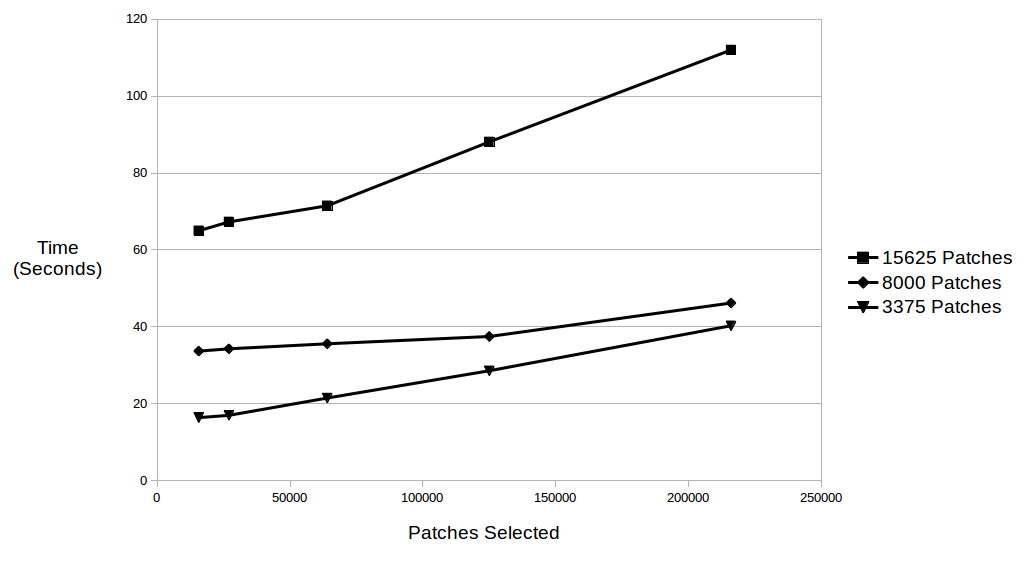
\includegraphics[scale=0.6]{area-select-graph}
\caption{A graph of the time taken to load different numbers of patches across different files}
\label{explore-graph}
\end{figure}

\section{Evaluation}

\subsection{Improvements}
\subsubsection{HDF5 Support}
In addition to the ASCII based Peano file format which our project supports, Peano also has a HDF5 Format \cite{hdf5}. A brief description of the two solutions is found below.

\textbf{Advantages of HDF5}
\begin{itemize}
\item HDF5 is both quicker to read and write to because time does not need to be spent converting values between character strings and binary floating-point values.
\item HDF5 requires less disk space because the character string representation of most floating point values is larger than the binary representation.
\end{itemize}

\textbf{Advantages of ASCII}
\begin{itemize}
\item The ASCII file format is directly human readable which makes it relatively easy to debug. However there are tools available such as HDF Explorer \cite{hdfexplorer} which can view the contents of HDF5 files.
\item HDF5 files need external libraries for read and write operations but the ASCII format does not.
\end{itemize}

The project was designed in such a way that support for the HDF5 file format is easily implementable by extending the $PeanoReader$ object to also read HDF5 patch files into the internal PeanoPatch objects.

\subsubsection{Sampling}
Sampling methods can be thought of as either forward or backward. A forward method populates the output dataset by iterating over all points in the input dataset and mapping them onto the output dataset. A backward method populates the output grid by iterating over all points in the output dataset and mapping them to input dataset. A backward method has the advantage that no points in the output grid will be unpopulated. An example of some points in the output grid being unpopulated can be found in the Problems section on page \pageref{blank-artifacts}.

The time complexity of a sampling method is $O(n \times f())$ where $n$ is the size of the dataset you are mapping from and $f()$ is the time complexity of mapping from a point in space to the nearest point in the dataset you are mapping to. The time complexities of $f()$ for different data structures are found in table \ref{time-complexities}.

\begin{table}[h]
\centering
\begin{tabular}{|l|l|}
\hline
\textbf{Data Type}                            & \textbf{Time Complexity} \\ \hline
Peano Patch (Regular Grid)             & $O(1)$            \\ \hline
Spacetree                              & $O(log(n))$       \\ \hline
Peano Patch Set (Set of Regular Grids) & $O(n)$            \\ \hline
\end{tabular}
\caption{Time complexity of mapping to a point in space to a point in the dataset}
\label{time-complexities}
\end{table}

The input dataset is a PeanoPatchSet and the output dataset is a Regular Grid. Therefore in order to minimize the time complexity we use forward mapping. This results in a time complexity of $O(n)$ where $n$ is the size of the input dataset.

When sampling on-the-fly from an already compressed dataset, the input dataset will be a PeanoPatch Set of size 1. This means it is equivalent to a regular grid and therefore the mapping operation can be performed in constant time. This means that if we were to use backward mapping, the operation could be performed in $O(m)$ time complexity where $m$ is the size of the output dataset. This would be a significant performance increase since in our use case, the output dataset is significantly smaller than the input dataset.


The sampling method we implemented is a type of forward sampling and so the time complexity is $O(n)$ where $n$ is the size of the output dataset. This is because the calculation of the mapping takes constant time and we iterate over every point in the input dataset once. For backward mapping, the time complexity depends on the structure of the input dataset. If the input dataset is a single regular grid (i.e. it has already been compressed) then the backward mapping can be performed in $O(m)$ run time where $m$ is the size of the output dataset. In the standard use case, this would create a performance benefit because the output dataset is smaller than the input dataset.
Sampling could be done backwards if the input dataset is a regular grid. This would transform the runtime from the size of the input dataset to the size of the output dataset.

\subsubsection{Parallelisation}
Currently this software implements little parallelisation. The standalone program will parallelize the low resolution computation by running each input dataset on its own thread. However this isn't ideal because if there are more cores available than there are datasets then some cores will not be utilized. Additionally, the memory usage is significantly increased because multiple input files are loaded at once. Instead, it would be more effective if the sampling method was parallelized. Since the number of points in the full resolution data is almost guarenteed to be larger than the number of cores it is unlikely that any cores will be unused. Additionally, only a single dataset will need to be loaded into memory at once, significantly reducing the memory footprint.



\subsection{Problems}
\subsubsection{Sampling}
When sampling the full resolution data on the a regular grid, if any part of the full resolution data has a lower resolution than the grid, then some cells or vertices of the output grid will not be populated. Currently there is no mechanism  implemented to detect if this occurs. Figure \ref{blank-artifacts} shows a regular $10 \times 10 \times 10$ grid where this has occured. The red cells were successfully sampled and the blue cells were not. This error does not occur if backward sampling is used instead.

\begin{figure}[h]
\centering
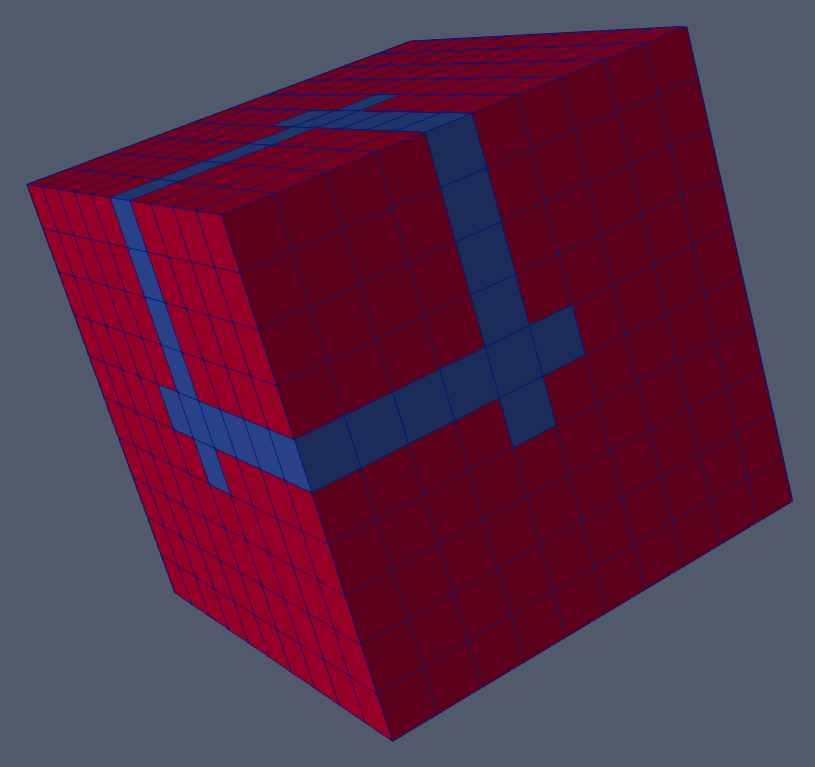
\includegraphics[scale=0.25]{data-artifacts}
\caption{The areas of a regular grid with no data sampled onto it (blue)}
\label{blank-artifacts}
\end{figure}

\subsubsection{Area Selection Interface}
The interface of the plugin has some issues which limit its usefulness. The sampling method only allows selection of areas which are aligned with the grid however it is possible to rotate the selection box by dragging on a face of the cube. This is because the box selection interface we used came from ParaView and full customization of it was not possible.

\section{Conclusions}

Through the extension of the Peano file format to support multiscale data and an interactive visual exploration plugin for ParaView, it is possible to explore massive datasets produced by ExaHyPE in real time while maintaing the visual quality requirements. The pre-computation of adequate low resolution versions provides enough detail for human researchers to understand the gist of the data. The interactive selection tool can be used to select areas of interest. There would be a significant performance benefit if the HDF5 Peano file format was supported and this project was designed with possible HDF5 integration in mind.

\subsection{Importance}
As the scientific community prepares for the arrival of exascale computational systems, it is vital that as much software and technology is prepared in advance as possible. This is so that any down time is minimized. This project, and projects like it are vital because the research that exascale computing will allow us to perform is useless if we are unable to actually consume the data they produce.

\subsection{Applications}
This project was started with a specific use case in mind; to significantly increase the ability for researchers to handle large data produced by ExaHyPE. However there are some other useful applications of this project. Some isosurface algorithms which create a 3D surfaces, such as Marching Cubes \cite{Lorensen:1987:MCH:37402.37422}, can only be performed on regular grids, so by first sampling the Peano patch data onto a regular grid we can extract an isosurface from the dataset.

\bibliography{projectpaper}


\end{document}
